\section{Álgebra booleana e funções (portas lógicas)}

\frame{
	\frametitle{Álgebra booleana}
	\centerline{\includegraphics[width=0.3\linewidth]{Figuras/Ch3/boole.png}}
	\begin{block}{Notação}
		\begin{itemize}
			\item ``1'' representa a classe de todos os objetos (o universo).
			\item ``0'' representa a classe a que nenhum objeto pertença (a classe vazia).
		\end{itemize}
	\end{block}
}

\frame{
	\frametitle{Portas lógicas - Introdução}
	
	\centering
	
	\setmyunit{2cm}
	
	\begin{circuitikz}
		\node[and port] (a1) at (3,0) {};
		\node[and port] (a2) at (3,-1) {};
		\node[or port] (o1) at (4,-0.5) {};
		\node[not port,scale=0.5] (n1) at (1.5,0 |- a1.in 1) {};
		\node[not port,scale=0.5] (n2) at (1.5,0 |- a2.in 2) {};
		
		\draw (a1.in 1 -| 0,0) ++(0,0.25) node[left,name=p1] {0} to[short, -*] ++(0.5,0) -| (n1.in)
			(n1.out) -| (a1.in 1)
			(a2.in 2 -| 0,0) ++(0,-0.25) node[left,name=p2] {0} to[short, -*] ++(0.25,0) -| (n2.in)
			(n2.out) --  (a2.in 2)
			(a1.in 2) -| (0.25,0 |- p2)
			(a2.in 1) -| (0.5,0 |- p1)
			(a1.out) -| (o1.in 1)
			(a2.out) -| (o1.in 2)
			(o1.out) -- +(0.5,0) node[right] {0};
	\end{circuitikz}
%	\centerline{\includegraphics[width=0.8\linewidth]{Figuras/Ch3/portas.png}}
}

\frame{
	\frametitle{Portas lógicas - Introdução}
	\begin{block}{O que são portas lógicas?}
		\begin{itemize}
			\item Blocos básicos.
			\item No mínimo: 1 entrada e 1 saída.
			\item Não possuem memória.
			\item Representação gráfica.
			\item Tabela verdade.
		\end{itemize}
	\end{block}
	\begin{block}{Nas funções lógicas há 2 valores:}
		\begin{itemize}
			\item $ 0 = $ Falso, sem tensão, baixo.
			\item $ 1 = $ Verdadeiro, com tensão, alto.
		\end{itemize}
	\end{block}
}

\frame{
	\frametitle{Portas lógicas - E (AND)}
	\begin{block}{Notação}
		\[ Y=A\cdot B \]
	\end{block}

	\bigskip
	
	\begin{minipage}{0.49\linewidth}
		\centering
		\renewcommand{\arraystretch}{1}
		\resizebox{0.6\textwidth}{!}{
			\begin{tabular}{cc|c}
				\toprule
				$ A $ & $ B $ & $ Y $ \\ \midrule
				0 & 0 & 0 \\
				0 & 1 & 0 \\
				1 & 0 & 0 \\
				1 & 1 & 1 \\ \bottomrule
		\end{tabular}}
	\end{minipage}
	\hfill
	\begin{minipage}{0.49\linewidth}
		
		\setmyunit{2cm}
		
		\centering
		\begin{circuitikz}
			\node[and port] (a) at (1,-0.5) {};
			\draw (0,0) node[left] {$ A $} -| (a.in 1)
			(0,-1) node[left] {$ B $} -| (a.in 2)
			(a.out) -- +(0.25,0) node[right] {$ Y $};
		\end{circuitikz}
	\end{minipage}
%	\centerline{\includegraphics[width=0.6\linewidth]{Figuras/Ch3/and.png}}
}

\frame{
	\frametitle{Portas lógicas - E (AND) - Circuito}
	
	\setmyunit{2cm}
	
	\centering
	\begin{circuitikz}
		\draw (0,0) to[battery,invert] ++(0,1) to[nos=$ A $] ++(1,0) to[nos=$ B $] ++(1,0) to[leDo,l_=$ Y $] ++(0,-1) -- ++(-2,0);
	\end{circuitikz}
%	\centerline{\includegraphics[width=0.6\linewidth]{Figuras/Ch3/andcirc.png}}
}

\frame{
	\frametitle{Portas lógicas - OU (OR)}
	\begin{block}{Notação}
		\[ Y=A+ B \]
	\end{block}
	
	\bigskip
	
	\begin{minipage}{0.49\linewidth}
		\centering
		\renewcommand{\arraystretch}{1}
		\resizebox{0.6\textwidth}{!}{
			\begin{tabular}{cc|c}
				\toprule
				$ A $ & $ B $ & $ Y $ \\ \midrule
				0 & 0 & 0 \\
				0 & 1 & 1 \\
				1 & 0 & 1 \\
				1 & 1 & 1 \\ \bottomrule
		\end{tabular}}
	\end{minipage}
	\hfill
	\begin{minipage}{0.49\linewidth}
		
		\setmyunit{2cm}
		
		\centering
		\begin{circuitikz}
			\node[or port] (a) at (1,-0.5) {};
			\draw (0,0) node[left] {$ A $} -| (a.in 1)
			(0,-1) node[left] {$ B $} -| (a.in 2)
			(a.out) -- +(0.25,0) node[right] {$ Y $};
		\end{circuitikz}
	\end{minipage}
%	\centerline{\includegraphics[width=0.6\linewidth]{Figuras/Ch3/or.png}}
}

\frame{
	\frametitle{Portas lógicas - OU (OR) - Circuito}
	
	\setmyunit{2cm}
	
	\centering
	\begin{circuitikz}
		\draw (0,0) to[battery,invert] ++(0,1) to[short,-*] ++(0.5,0) -- ++(0,0.25) to[nos=$ A $] ++(1,0) -- ++(0,-0.25) to[short,-*] ++(0,-0.25) to[nos,l_=$ B $,invert,mirror] ++(-1,0) -- ++(0,0.25) ++(1,0) -- ++(0.5,0) to[leDo,l_=$ Y $] ++(0,-1) -- ++(-2,0);
	\end{circuitikz}
%	\centerline{\includegraphics[width=0.6\linewidth]{Figuras/Ch3/orcirc.png}}
}

\frame{
	\frametitle{Portas lógicas - NÃO (NOT)}
	\begin{block}{Notação}
		\[ Y=\notted{A} \]
	\end{block}
	
	\bigskip
	
	\begin{minipage}{0.49\linewidth}
		\centering
		\renewcommand{\arraystretch}{1}
		\resizebox{0.4\textwidth}{!}{
			\begin{tabular}{c|c}
				\toprule
				$ A $ & $ Y $ \\ \midrule
				1 & 0 \\
				0 & 1 \\ \bottomrule
		\end{tabular}}
	\end{minipage}
	\hfill
	\begin{minipage}{0.49\linewidth}
		
		\setmyunit{2cm}
		
		\centering
		\begin{circuitikz}
			\node[not port] (a) at (1,-0.5) {};
			\draw (a.in) -- +(-0.25,0) node[left] {$ A $} (a.out) -- +(0.25,0) node[right] {$ Y $};
		\end{circuitikz}
	\end{minipage}
%	\centerline{\includegraphics[width=0.6\linewidth]{Figuras/Ch3/not.png}}
}

\frame{
	\frametitle{Portas lógicas - NÃO (NOT) - Circuito}
	\setmyunit{2cm}
	\centering
	\begin{circuitikz}
		\draw (0,0) to[battery,invert] ++(0,1) to[R=$ R $] ++(1,0) to[nos=$ A $,*-*] ++(0,-1) -- ++(1,0) to[leDo,invert,l_=$ Y $] ++(0,1) -- ++(-1,0) ++(0,-1) -- ++(-1,0);
	\end{circuitikz}
%	\centerline{\includegraphics[width=0.6\linewidth]{Figuras/Ch3/notcirc.PNG}}
}

\frame{
	\frametitle{Portas lógicas - NÃO E (NAND)}
	\begin{block}{Notação}
		\[ Y=\notted{A\cdot B} \]
	\end{block}
	
	\bigskip
	
	\begin{minipage}{0.49\linewidth}
		\centering
		\renewcommand{\arraystretch}{1}
		\resizebox{0.6\textwidth}{!}{
			\begin{tabular}{cc|c}
				\toprule
				$ A $ & $ B $ & $ Y $ \\ \midrule
				0 & 0 & 1 \\
				0 & 1 & 1 \\
				1 & 0 & 1 \\
				1 & 1 & 0 \\ \bottomrule
		\end{tabular}}
	\end{minipage}
	\hfill
	\begin{minipage}{0.49\linewidth}
		
		\setmyunit{2cm}
		
		\centering
		\begin{circuitikz}
			\node[nand port] (a) at (1,-0.5) {};
			\draw (0,0) node[left] {$ A $} -| (a.in 1)
			(0,-1) node[left] {$ B $} -| (a.in 2)
			(a.out) -- +(0.25,0) node[right] {$ Y $};
		\end{circuitikz}
	\end{minipage}
%	\centerline{\includegraphics[width=0.6\linewidth]{Figuras/Ch3/nand.png}}
}

\frame{
	\frametitle{Portas lógicas - NÃO E (NAND) - Circuito}
%	\setmyunit{2cm}
	\centering
	\begin{circuitikz}[x=3cm,y=1.5cm]
		\draw (0,0) to[battery, invert] ++(0,2) to[R=$ R $] ++(1,0) to[nos=$ A $, *-] ++(0,-1) to[nos=$ B $,-*] ++(0,-1) ++(0,2) -- ++(1,0) to[leDo,l_=$ Y $] ++(0,-2) -- ++(-2,0);
	\end{circuitikz}
%	\centerline{\includegraphics[width=0.6\linewidth]{Figuras/Ch3/nandcirc.png}}
}

\frame{
	\frametitle{Portas lógicas - NÃO OU (NOR)}
	\begin{block}{Notação}
		\[ Y=\notted{A\cdot B} \]
	\end{block}
	
	\bigskip
	
	\begin{minipage}{0.49\linewidth}
		\centering
		\renewcommand{\arraystretch}{1}
		\resizebox{0.6\textwidth}{!}{
			\begin{tabular}{cc|c}
				\toprule
				$ A $ & $ B $ & $ Y $ \\ \midrule
				0 & 0 & 1 \\
				0 & 1 & 0 \\
				1 & 0 & 0 \\
				1 & 1 & 0 \\ \bottomrule
		\end{tabular}}
	\end{minipage}
	\hfill
	\begin{minipage}{0.49\linewidth}
		
		\setmyunit{2cm}
		
		\centering
		\begin{circuitikz}
			\node[nor port] (a) at (1,-0.5) {};
			\draw (0,0) node[left] {$ A $} -| (a.in 1)
			(0,-1) node[left] {$ B $} -| (a.in 2)
			(a.out) -- +(0.25,0) node[right] {$ Y $};
		\end{circuitikz}
	\end{minipage}
%	\centerline{\includegraphics[width=0.6\linewidth]{Figuras/Ch3/nor.png}}
}

\frame{
	\frametitle{Portas lógicas - NÃO OU (NOR) - Circuito}
	%	\setmyunit{2cm}
	\centering
	\begin{circuitikz}[x=4cm,y=2cm]
		\draw (0,0) to[battery, invert] ++(0,1) to[R=$ R $] ++(0.5,0) to[nos=$ A $, *-*] ++(0,-1) ++(0,1) -- ++(0.5,0) to[nos=$ B $,*-*] ++(0,-1) ++(0,1) -- ++(0.5,0) to[leDo,l_=$ Y $] ++(0,-1) -- ++(-1.5,0);
	\end{circuitikz}
%	\centerline{\includegraphics[width=0.6\linewidth]{Figuras/Ch3/norcirc.PNG}}
}

\frame{
	\frametitle{Portas lógicas - OU EXCLUSIVO (XOR)}
	\begin{block}{Notação}
		\[ Y=A\oplus B \]
	\end{block}
	
	\bigskip
	
	\begin{minipage}{0.49\linewidth}
		\centering
		\renewcommand{\arraystretch}{1}
		\resizebox{0.6\textwidth}{!}{
			\begin{tabular}{cc|c}
				\toprule
				$ A $ & $ B $ & $ Y $ \\ \midrule
				0 & 0 & 0 \\
				0 & 1 & 1 \\
				1 & 0 & 1 \\
				1 & 1 & 0 \\ \bottomrule
		\end{tabular}}
	\end{minipage}
	\hfill
	\begin{minipage}{0.49\linewidth}
		
		\setmyunit{2cm}
		
		\centering
		\begin{circuitikz}
			\node[xor port] (a) at (1,-0.5) {};
			\draw (0,0) node[left] {$ A $} -| (a.in 1)
			(0,-1) node[left] {$ B $} -| (a.in 2)
			(a.out) -- +(0.25,0) node[right] {$ Y $};
		\end{circuitikz}
	\end{minipage}
%	\centerline{\includegraphics[width=0.6\linewidth]{Figuras/Ch3/xor.png}}
}

\frame{
	\frametitle{Portas lógicas - COINCIDÊNCIA (XNOR)}
	\begin{block}{Notação}
		\[ Y=\notted{A\oplus B}=A\odot B \]
	\end{block}
	
	\bigskip
	
	\begin{minipage}{0.49\linewidth}
		\centering
		\renewcommand{\arraystretch}{1}
		\resizebox{0.6\textwidth}{!}{
			\begin{tabular}{cc|c}
				\toprule
				$ A $ & $ B $ & $ Y $ \\ \midrule
				0 & 0 & 1 \\
				0 & 1 & 0 \\
				1 & 0 & 0 \\
				1 & 1 & 1 \\ \bottomrule
		\end{tabular}}
	\end{minipage}
	\hfill
	\begin{minipage}{0.49\linewidth}
		
		\setmyunit{2cm}
		
		\centering
		\begin{circuitikz}
			\node[xnor port] (a) at (1,-0.5) {};
			\draw (0,0) node[left] {$ A $} -| (a.in 1)
			(0,-1) node[left] {$ B $} -| (a.in 2)
			(a.out) -- +(0.25,0) node[right] {$ Y $};
		\end{circuitikz}
	\end{minipage}
%	\centerline{\includegraphics[width=0.6\linewidth]{Figuras/Ch3/xnor.png}}
}

\frame{
	\frametitle{Portas universais}
	\begin{block}{NAND e NOR são portas universais}
		É possível obter a partir delas as portas:
		\begin{itemize}
			\item NOT
			\item AND
			\item OR
		\end{itemize}

		\centering \textbf{APOSTILA!}
	\end{block}
}

\section*{Exercícios}
\frame{
	\frametitle{Exercícios}

	\begin{block}{}
		01. Desenhe a forma de onda de saída para uma porta NOR.

		\begin{itemize}
			\item Repita para a entrada C mantida sempre em nível baixo.
			\item Repita para a entrada C mantida sempre em nível alto.
		\end{itemize}

		02. Repita o problema para uma porta NAND.
	\end{block}
	
	\medskip
	
	\centering
	

\tikzset{every picture/.style={line width=0.75pt}} %set default line width to 0.75pt        

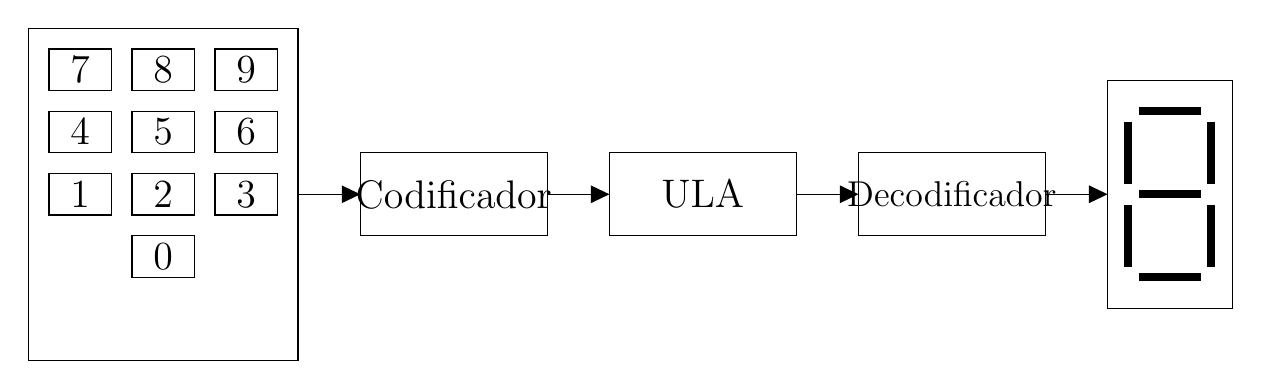
\begin{tikzpicture}[x=0.75pt,y=0.75pt,yscale=-1,xscale=1]
%uncomment if require: \path (0,300); %set diagram left start at 0, and has height of 300

%Shape: Rectangle [id:dp8798188650405219] 
\draw   (30,50) -- (160,50) -- (160,210) -- (30,210) -- cycle ;
%Shape: Rectangle [id:dp593444354888008] 
\draw   (40,60) -- (70,60) -- (70,80) -- (40,80) -- cycle ;
%Shape: Rectangle [id:dp4412846627526852] 
\draw   (80,60) -- (110,60) -- (110,80) -- (80,80) -- cycle ;
%Shape: Rectangle [id:dp2343273962035186] 
\draw   (120,60) -- (150,60) -- (150,80) -- (120,80) -- cycle ;
%Shape: Rectangle [id:dp05777918912875246] 
\draw   (40,90) -- (70,90) -- (70,110) -- (40,110) -- cycle ;
%Shape: Rectangle [id:dp9955010424516375] 
\draw   (80,90) -- (110,90) -- (110,110) -- (80,110) -- cycle ;
%Shape: Rectangle [id:dp24021539717259266] 
\draw   (120,90) -- (150,90) -- (150,110) -- (120,110) -- cycle ;
%Shape: Rectangle [id:dp36169684584711925] 
\draw   (40,120) -- (70,120) -- (70,140) -- (40,140) -- cycle ;
%Shape: Rectangle [id:dp7232437677097003] 
\draw   (80,120) -- (110,120) -- (110,140) -- (80,140) -- cycle ;
%Shape: Rectangle [id:dp6884539525496838] 
\draw   (120,120) -- (150,120) -- (150,140) -- (120,140) -- cycle ;
%Shape: Rectangle [id:dp9961423077173726] 
\draw   (80,150) -- (110,150) -- (110,170) -- (80,170) -- cycle ;
%Shape: Rectangle [id:dp6643057105712631] 
\draw   (190,110) -- (280,110) -- (280,150) -- (190,150) -- cycle ;
%Shape: Rectangle [id:dp7094011053258715] 
\draw   (550,75) -- (610,75) -- (610,185) -- (550,185) -- cycle ;
%Shape: Rectangle [id:dp2693438921699036] 
\draw   (310,110) -- (400,110) -- (400,150) -- (310,150) -- cycle ;
%Shape: Rectangle [id:dp3654960401722005] 
\draw   (430,110) -- (520,110) -- (520,150) -- (430,150) -- cycle ;
%Straight Lines [id:da6667328032348829] 
\draw    (160,130) -- (188,130) ;
\draw [shift={(190,130)}, rotate = 180] [fill={rgb, 255:red, 0; green, 0; blue, 0 }  ][line width=0.75]  [draw opacity=0] (8.93,-4.29) -- (0,0) -- (8.93,4.29) -- cycle    ;

%Straight Lines [id:da5165651690517046] 
\draw    (280,130) -- (308,130) ;
\draw [shift={(310,130)}, rotate = 180] [fill={rgb, 255:red, 0; green, 0; blue, 0 }  ][line width=0.75]  [draw opacity=0] (8.93,-4.29) -- (0,0) -- (8.93,4.29) -- cycle    ;

%Straight Lines [id:da17751850693095572] 
\draw    (400,130) -- (428,130) ;
\draw [shift={(430,130)}, rotate = 180] [fill={rgb, 255:red, 0; green, 0; blue, 0 }  ][line width=0.75]  [draw opacity=0] (8.93,-4.29) -- (0,0) -- (8.93,4.29) -- cycle    ;

%Straight Lines [id:da4998570413390182] 
\draw [color={rgb, 255:red, 0; green, 0; blue, 0 }  ,draw opacity=1 ][line width=3]    (560,95) -- (560,125) ;


%Straight Lines [id:da05287212083080073] 
\draw [color={rgb, 255:red, 0; green, 0; blue, 0 }  ,draw opacity=1 ][line width=3]    (600,95) -- (600,125) ;


%Straight Lines [id:da9146969001147236] 
\draw [color={rgb, 255:red, 0; green, 0; blue, 0 }  ,draw opacity=1 ][line width=3]    (560,135) -- (560,165) ;


%Straight Lines [id:da37610179690179124] 
\draw [color={rgb, 255:red, 0; green, 0; blue, 0 }  ,draw opacity=1 ][line width=3]    (600,135) -- (600,165) ;


%Straight Lines [id:da2798262228013664] 
\draw [color={rgb, 255:red, 0; green, 0; blue, 0 }  ,draw opacity=1 ][line width=3]    (595,130) -- (565,130) ;


%Straight Lines [id:da15184615547446478] 
\draw [color={rgb, 255:red, 0; green, 0; blue, 0 }  ,draw opacity=1 ][line width=3]    (595,90) -- (565,90) ;


%Straight Lines [id:da20609816632014244] 
\draw [color={rgb, 255:red, 0; green, 0; blue, 0 }  ,draw opacity=1 ][line width=3]    (595,170) -- (565,170) ;


%Straight Lines [id:da16937059284664002] 
\draw    (520,130) -- (548,130) ;
\draw [shift={(550,130)}, rotate = 180] [fill={rgb, 255:red, 0; green, 0; blue, 0 }  ][line width=0.75]  [draw opacity=0] (8.93,-4.29) -- (0,0) -- (8.93,4.29) -- cycle    ;


% Text Node
\draw (135,70) node   {\Large $9$};
% Text Node
\draw (95,70) node   {\Large $8$};
% Text Node
\draw (55,70) node   {\Large $7$};
% Text Node
\draw (135,100) node   {\Large $6$};
% Text Node
\draw (135,130) node   {\Large $3$};
% Text Node
\draw (95,160) node   {\Large $0$};
% Text Node
\draw (95,130) node   {\Large $2$};
% Text Node
\draw (95,100) node   {\Large $5$};
% Text Node
\draw (55,100) node   {\Large $4$};
% Text Node
\draw (55,130) node   {\Large $1$};
% Text Node
\draw (235,130) node  [align=left] {\Large Codificador};
% Text Node
\draw (355,130) node  [align=left] {\Large ULA};
% Text Node
\draw (475,130) node [scale=0.9] [align=left] {\Large Decodificador};


\end{tikzpicture}

%	\centerline{\includegraphics[width=0.75\linewidth]{Figuras/Ch3/exerc.PNG}}
}


\section*{Referências}

\frame{
	\frametitle{Referências e exercícios complementares}
	\begin{itemize}
		\item IDOETA, Ivan V. e CAPUANO, Francisco G. Elementos de Eletrônica Digital. São Paulo:
		      Editora Érica, ed. 40. 2008.
	\end{itemize}
	\centering{\alert{Página 82 - \textbf{2.9.1, 2.9.14, 2.9.18 até 2.9.22}}}

}